\documentclass[14pt]{extbook}
\usepackage{multicol, enumerate, enumitem, hyperref, color, soul, setspace, parskip, fancyhdr} %General Packages
\usepackage{amssymb, amsthm, amsmath, bbm, latexsym, units, mathtools} %Math Packages
\everymath{\displaystyle} %All math in Display Style
% Packages with additional options
\usepackage[headsep=0.5cm,headheight=12pt, left=1 in,right= 1 in,top= 1 in,bottom= 1 in]{geometry}
\usepackage[usenames,dvipsnames]{xcolor}
\usepackage{dashrule}  % Package to use the command below to create lines between items
\newcommand{\litem}[1]{\item#1\hspace*{-1cm}\rule{\textwidth}{0.4pt}}
\pagestyle{fancy}
\lhead{Progress Quiz 4}
\chead{}
\rhead{Version A}
\lfoot{4378-7085}
\cfoot{}
\rfoot{Fall 2020}
\begin{document}

\begin{enumerate}
\litem{
Write the equation of the line in the graph below in Standard form $Ax+By=C$. Then, choose the intervals that contain $A, B, \text{ and } C$.
\begin{center}
    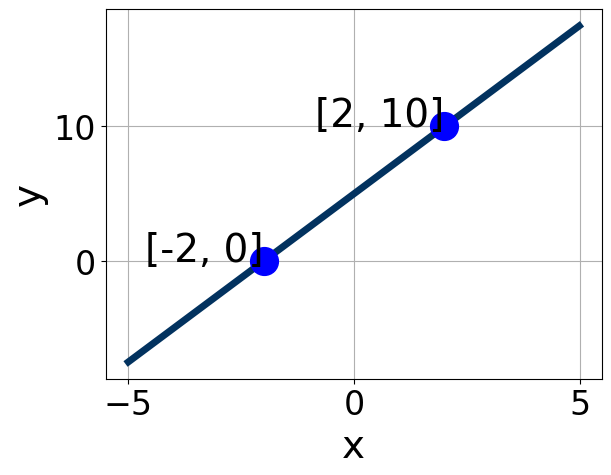
\includegraphics[width=0.5\textwidth]{../Figures/linearGraphToStandardCopyA.png}
\end{center}
\begin{enumerate}[label=\Alph*.]
\item \( A \in [3, 9], \hspace{3mm} B \in [-5.7, -2.2], \text{ and } \hspace{3mm} C \in [11, 21] \)
\item \( A \in [3, 9], \hspace{3mm} B \in [1.3, 5.7], \text{ and } \hspace{3mm} C \in [-16, -9] \)
\item \( A \in [-4.67, -0.67], \hspace{3mm} B \in [0.7, 2.2], \text{ and } \hspace{3mm} C \in [-6, 0] \)
\item \( A \in [-8, -4], \hspace{3mm} B \in [1.3, 5.7], \text{ and } \hspace{3mm} C \in [-16, -9] \)
\item \( A \in [-4.67, -0.67], \hspace{3mm} B \in [-2.9, 0.5], \text{ and } \hspace{3mm} C \in [5, 11] \)

\end{enumerate} }
\litem{
Solve the linear equation below. Then, choose the interval that contains the solution.\[ \frac{3x + 9}{2} - \frac{7x + 3}{3} = \frac{3x + 7}{8} \]\begin{enumerate}[label=\Alph*.]
\item \( x \in [-1.2, -0.1] \)
\item \( x \in [2.6, 4.2] \)
\item \( x \in [-0.7, 0.8] \)
\item \( x \in [1, 2.6] \)
\item \( \text{There are no real solutions.} \)

\end{enumerate} }
\litem{
Solve the equation below. Then, choose the interval that contains the solution.\[ -7(5x -18) = -8(-9x + 6) \]\begin{enumerate}[label=\Alph*.]
\item \( x \in [1.55, 2.74] \)
\item \( x \in [-2.29, -1.81] \)
\item \( x \in [0.36, 0.96] \)
\item \( x \in [-1.77, -0.42] \)
\item \( \text{There are no real solutions.} \)

\end{enumerate} }
\litem{
Write the equation of the line in the graph below in Standard form $Ax+By=C$. Then, choose the intervals that contain $A, B, \text{ and } C$.
\begin{center}
    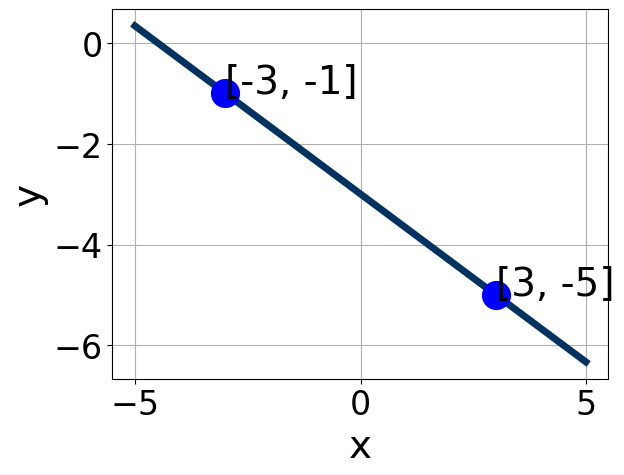
\includegraphics[width=0.5\textwidth]{../Figures/linearGraphToStandardA.png}
\end{center}
\begin{enumerate}[label=\Alph*.]
\item \( A \in [0.68, 2.02], \hspace{3mm} B \in [2.54, 3.39], \text{ and } \hspace{3mm} C \in [-12, -8] \)
\item \( A \in [0.68, 2.02], \hspace{3mm} B \in [-3.4, -1.98], \text{ and } \hspace{3mm} C \in [7, 10] \)
\item \( A \in [-2.64, -0.91], \hspace{3mm} B \in [-3.4, -1.98], \text{ and } \hspace{3mm} C \in [7, 10] \)
\item \( A \in [-0.59, 1.1], \hspace{3mm} B \in [0.46, 1.56], \text{ and } \hspace{3mm} C \in [-3, -1] \)
\item \( A \in [-0.59, 1.1], \hspace{3mm} B \in [-1.28, -0.97], \text{ and } \hspace{3mm} C \in [3, 7] \)

\end{enumerate} }
\litem{
First, find the equation of the line containing the two points below. Then, write the equation as $ y=mx+b $ and choose the intervals that contain $m$ and $b$.\[ (11, -9) \text{ and } (-6, -7) \]\begin{enumerate}[label=\Alph*.]
\item \( m \in [-0.12, -0.04] \hspace*{3mm} b \in [-22, -19] \)
\item \( m \in [-0.12, -0.04] \hspace*{3mm} b \in [4.71, 11.71] \)
\item \( m \in [0.09, 0.32] \hspace*{3mm} b \in [-7.29, -1.29] \)
\item \( m \in [-0.12, -0.04] \hspace*{3mm} b \in [-1, 4] \)
\item \( m \in [-0.12, -0.04] \hspace*{3mm} b \in [-10.71, -6.71] \)

\end{enumerate} }
\litem{
Solve the linear equation below. Then, choose the interval that contains the solution.\[ \frac{6x + 5}{5} - \frac{-6x -8}{7} = \frac{7x -6}{3} \]\begin{enumerate}[label=\Alph*.]
\item \( x \in [-0.83, 0.17] \)
\item \( x \in [67.79, 72.79] \)
\item \( x \in [12, 18] \)
\item \( x \in [5.72, 7.72] \)
\item \( \text{There are no real solutions.} \)

\end{enumerate} }
\litem{
Solve the equation below. Then, choose the interval that contains the solution.\[ -11(-18x -10) = -16(13x -6) \]\begin{enumerate}[label=\Alph*.]
\item \( x \in [0.36, 0.79] \)
\item \( x \in [-0.88, -0.32] \)
\item \( x \in [20.04, 21.19] \)
\item \( x \in [-0.17, 0.33] \)
\item \( \text{There are no real solutions.} \)

\end{enumerate} }
\litem{
Find the equation of the line described below. Write the linear equation as $ y=mx+b $ and choose the intervals that contain $m$ and $b$.\[ \text{Parallel to } 3 x - 7 y = 13 \text{ and passing through the point } (-9, -3). \]\begin{enumerate}[label=\Alph*.]
\item \( m \in [-0.21, 0.83] \hspace*{3mm} b \in [0.5, 1.7] \)
\item \( m \in [-0.21, 0.83] \hspace*{3mm} b \in [4.1, 8] \)
\item \( m \in [2.31, 2.73] \hspace*{3mm} b \in [0.5, 1.7] \)
\item \( m \in [-0.21, 0.83] \hspace*{3mm} b \in [-2.1, 0.8] \)
\item \( m \in [-0.52, -0.34] \hspace*{3mm} b \in [-7.5, -4.8] \)

\end{enumerate} }
\litem{
First, find the equation of the line containing the two points below. Then, write the equation as $ y=mx+b $ and choose the intervals that contain $m$ and $b$.\[ (-6, 6) \text{ and } (3, -5) \]\begin{enumerate}[label=\Alph*.]
\item \( m \in [-0.9, 3.5] \hspace*{3mm} b \in [-9.22, -8.26] \)
\item \( m \in [-1.6, 0.7] \hspace*{3mm} b \in [10.79, 13.35] \)
\item \( m \in [-1.6, 0.7] \hspace*{3mm} b \in [1.29, 1.9] \)
\item \( m \in [-1.6, 0.7] \hspace*{3mm} b \in [-1.52, -1] \)
\item \( m \in [-1.6, 0.7] \hspace*{3mm} b \in [-8.05, -6.67] \)

\end{enumerate} }
\litem{
Find the equation of the line described below. Write the linear equation as $ y=mx+b $ and choose the intervals that contain $m$ and $b$.\[ \text{Parallel to } 8 x + 3 y = 9 \text{ and passing through the point } (-6, -2). \]\begin{enumerate}[label=\Alph*.]
\item \( m \in [-5.1, -2.5] \hspace*{3mm} b \in [17, 19] \)
\item \( m \in [-1, 0] \hspace*{3mm} b \in [-20, -14] \)
\item \( m \in [-5.1, -2.5] \hspace*{3mm} b \in [1, 7] \)
\item \( m \in [-5.1, -2.5] \hspace*{3mm} b \in [-20, -14] \)
\item \( m \in [2, 4.3] \hspace*{3mm} b \in [9, 16] \)

\end{enumerate} }
\end{enumerate}

\end{document}